\section{Methodology}

%IT HAS 8K keys!  How did we take these measurements
We instrumented ParSplice with performance counters and keyspace counters.  The
performance counters track ParSplice activities while keyspace counters track
which keys are being accessed by the ranks. Because the keyspace counters have
high overhead, we only turn them on for the following analysis.

\subsection{ParSplice Keyspace Analysis}

In the following section, we examine the keyspace size and access patterns
using Figures~\ref{fig:futurework-regimes} and~\ref{fig:methodology-keyspace}.

\subsubsection*{An active but small keyspace} The black text annotations in
Figure~\ref{fig:methodology-keyspace} show that the keyspace size ranges from
about 10K keys for 32 workers to 100K keys for 1048 workers.  The bars show
\(50-100\times\) as many reads (\texttt{get()}) as writes (\texttt{put()}).
Workers pull the same key for extended periods because the trajectory segment
is stuck in a deep state, so many coordinates are needed before the trajectory
moves on. Writes only occur for the final state of segments generated by
workers; their magnitude is smaller than reads because the caches ignore
redundant put requests. The number of read and write requests are highest at
the beginning of the run when workers generate segements for the same state,
which is cheap.

\subsubsection*{Entropy increases over time} The reads per second in
Figure~\ref{fig:futurework-regimes} show that the number of requests decreases
and the number of active keys increases over time. The resulting imbalance for
the two growth rates in Figure~\ref{fig:futurework-regimes} are shown in
Figure~\ref{fig:methodology-keys}, where reads are plotted for each unique
state (\(x\) axis). Keys are more popular than others (up to \(5\times\))
because workers start generating states with different coordinates later in the
run.

\subsubsection*{Entropy growth is structured} The access patterns reflect the
locality of computation: workers stuck in state basins generate segments with
similar coordinates. The growth rate, temperature, and number of workers
changes that locality, which has an effect on the structure of the keyspace.
Figure~\ref{fig:methodology-keys} shows that the number of reads changes with
different growth rates, but that spatial locality is similiar ({\it e.g.}, some
keys are stil \(5\times\) more popular than others).
Figure~\ref{fig:futurework-regimes} shows how entropy for different growth
rates has temporal locality, as the reads per second for 1M looks like the
reads per second for 100K stretched out along the time axis.  Trends also exist
for temperature and number of workers but are ommitted here for space. This
structure means that we can learn the regimes and adapt the storage system to
it. 

\begin{figure}[tbh]
  \noindent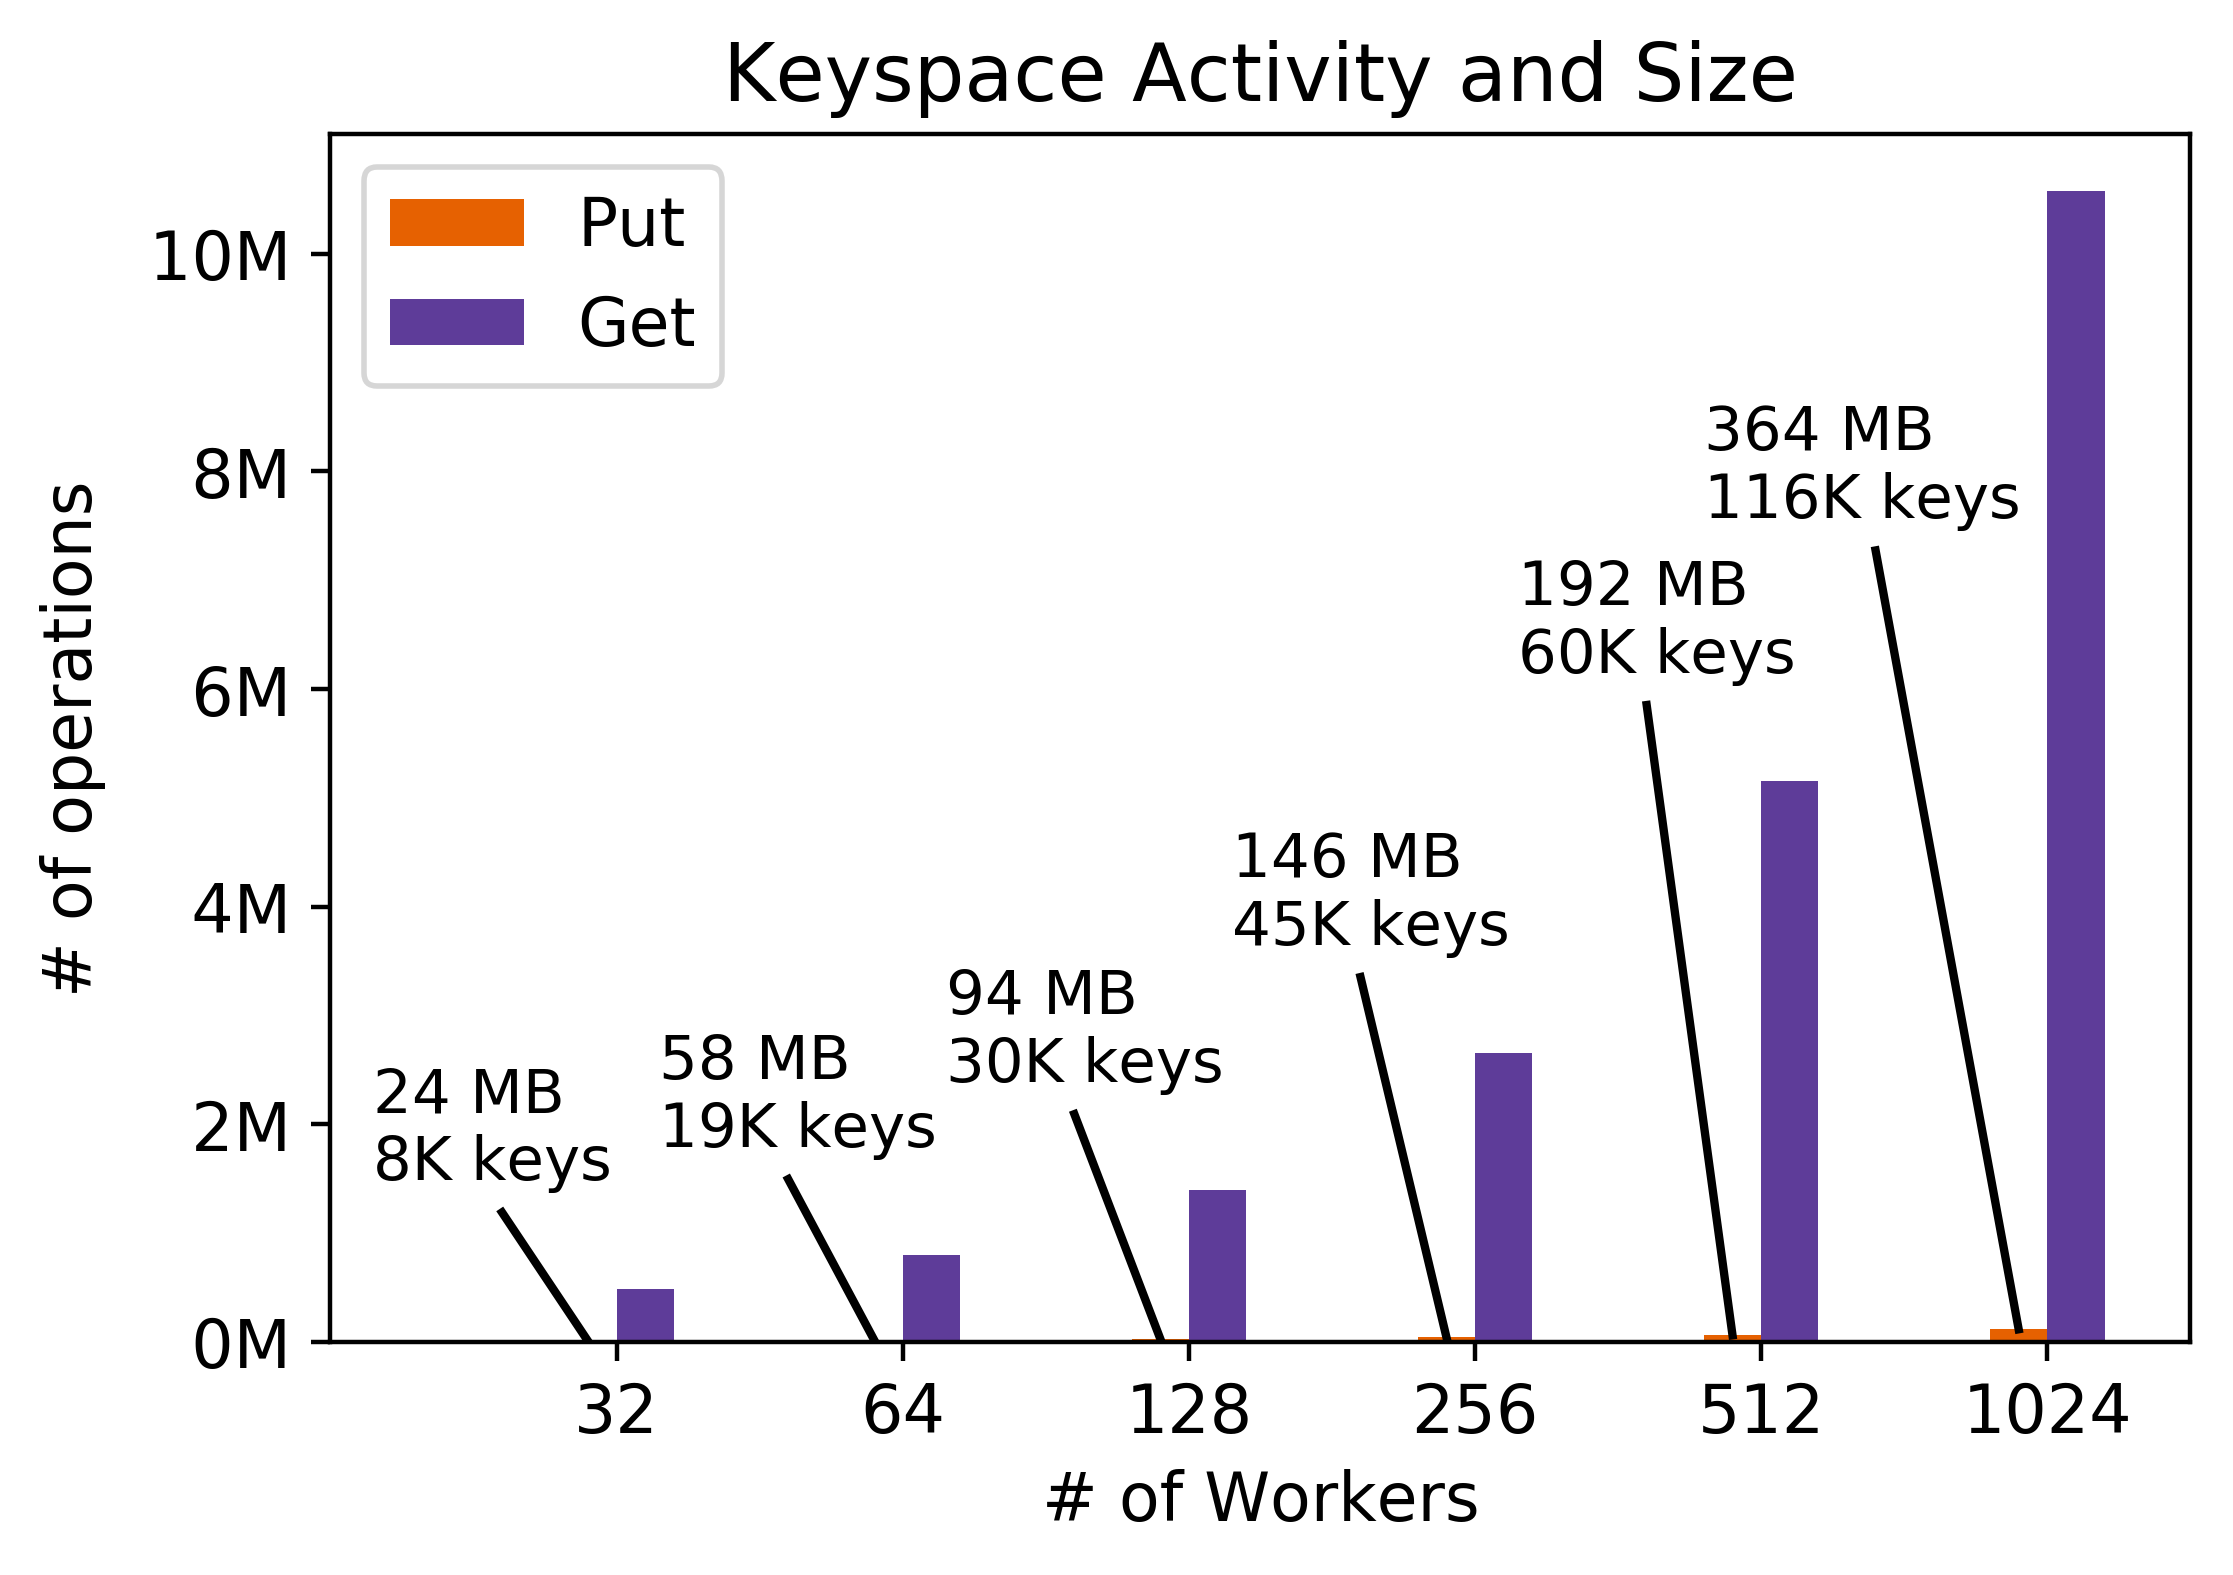
\includegraphics[width=0.45\textwidth]{figures/methodology-keyspace.png}\\
  \caption{The keyspace size is small (numbers above bars) but must
  satisfy many reads as workers calculate new segments. The active keyspace is
  difficult to predict a priori but the optimal load balancing strategy strikes a
  good balance between preformance and utilization. 
  \label{fig:methodology-keyspace}}
\end{figure}

\begin{figure}[tbh]
  \noindent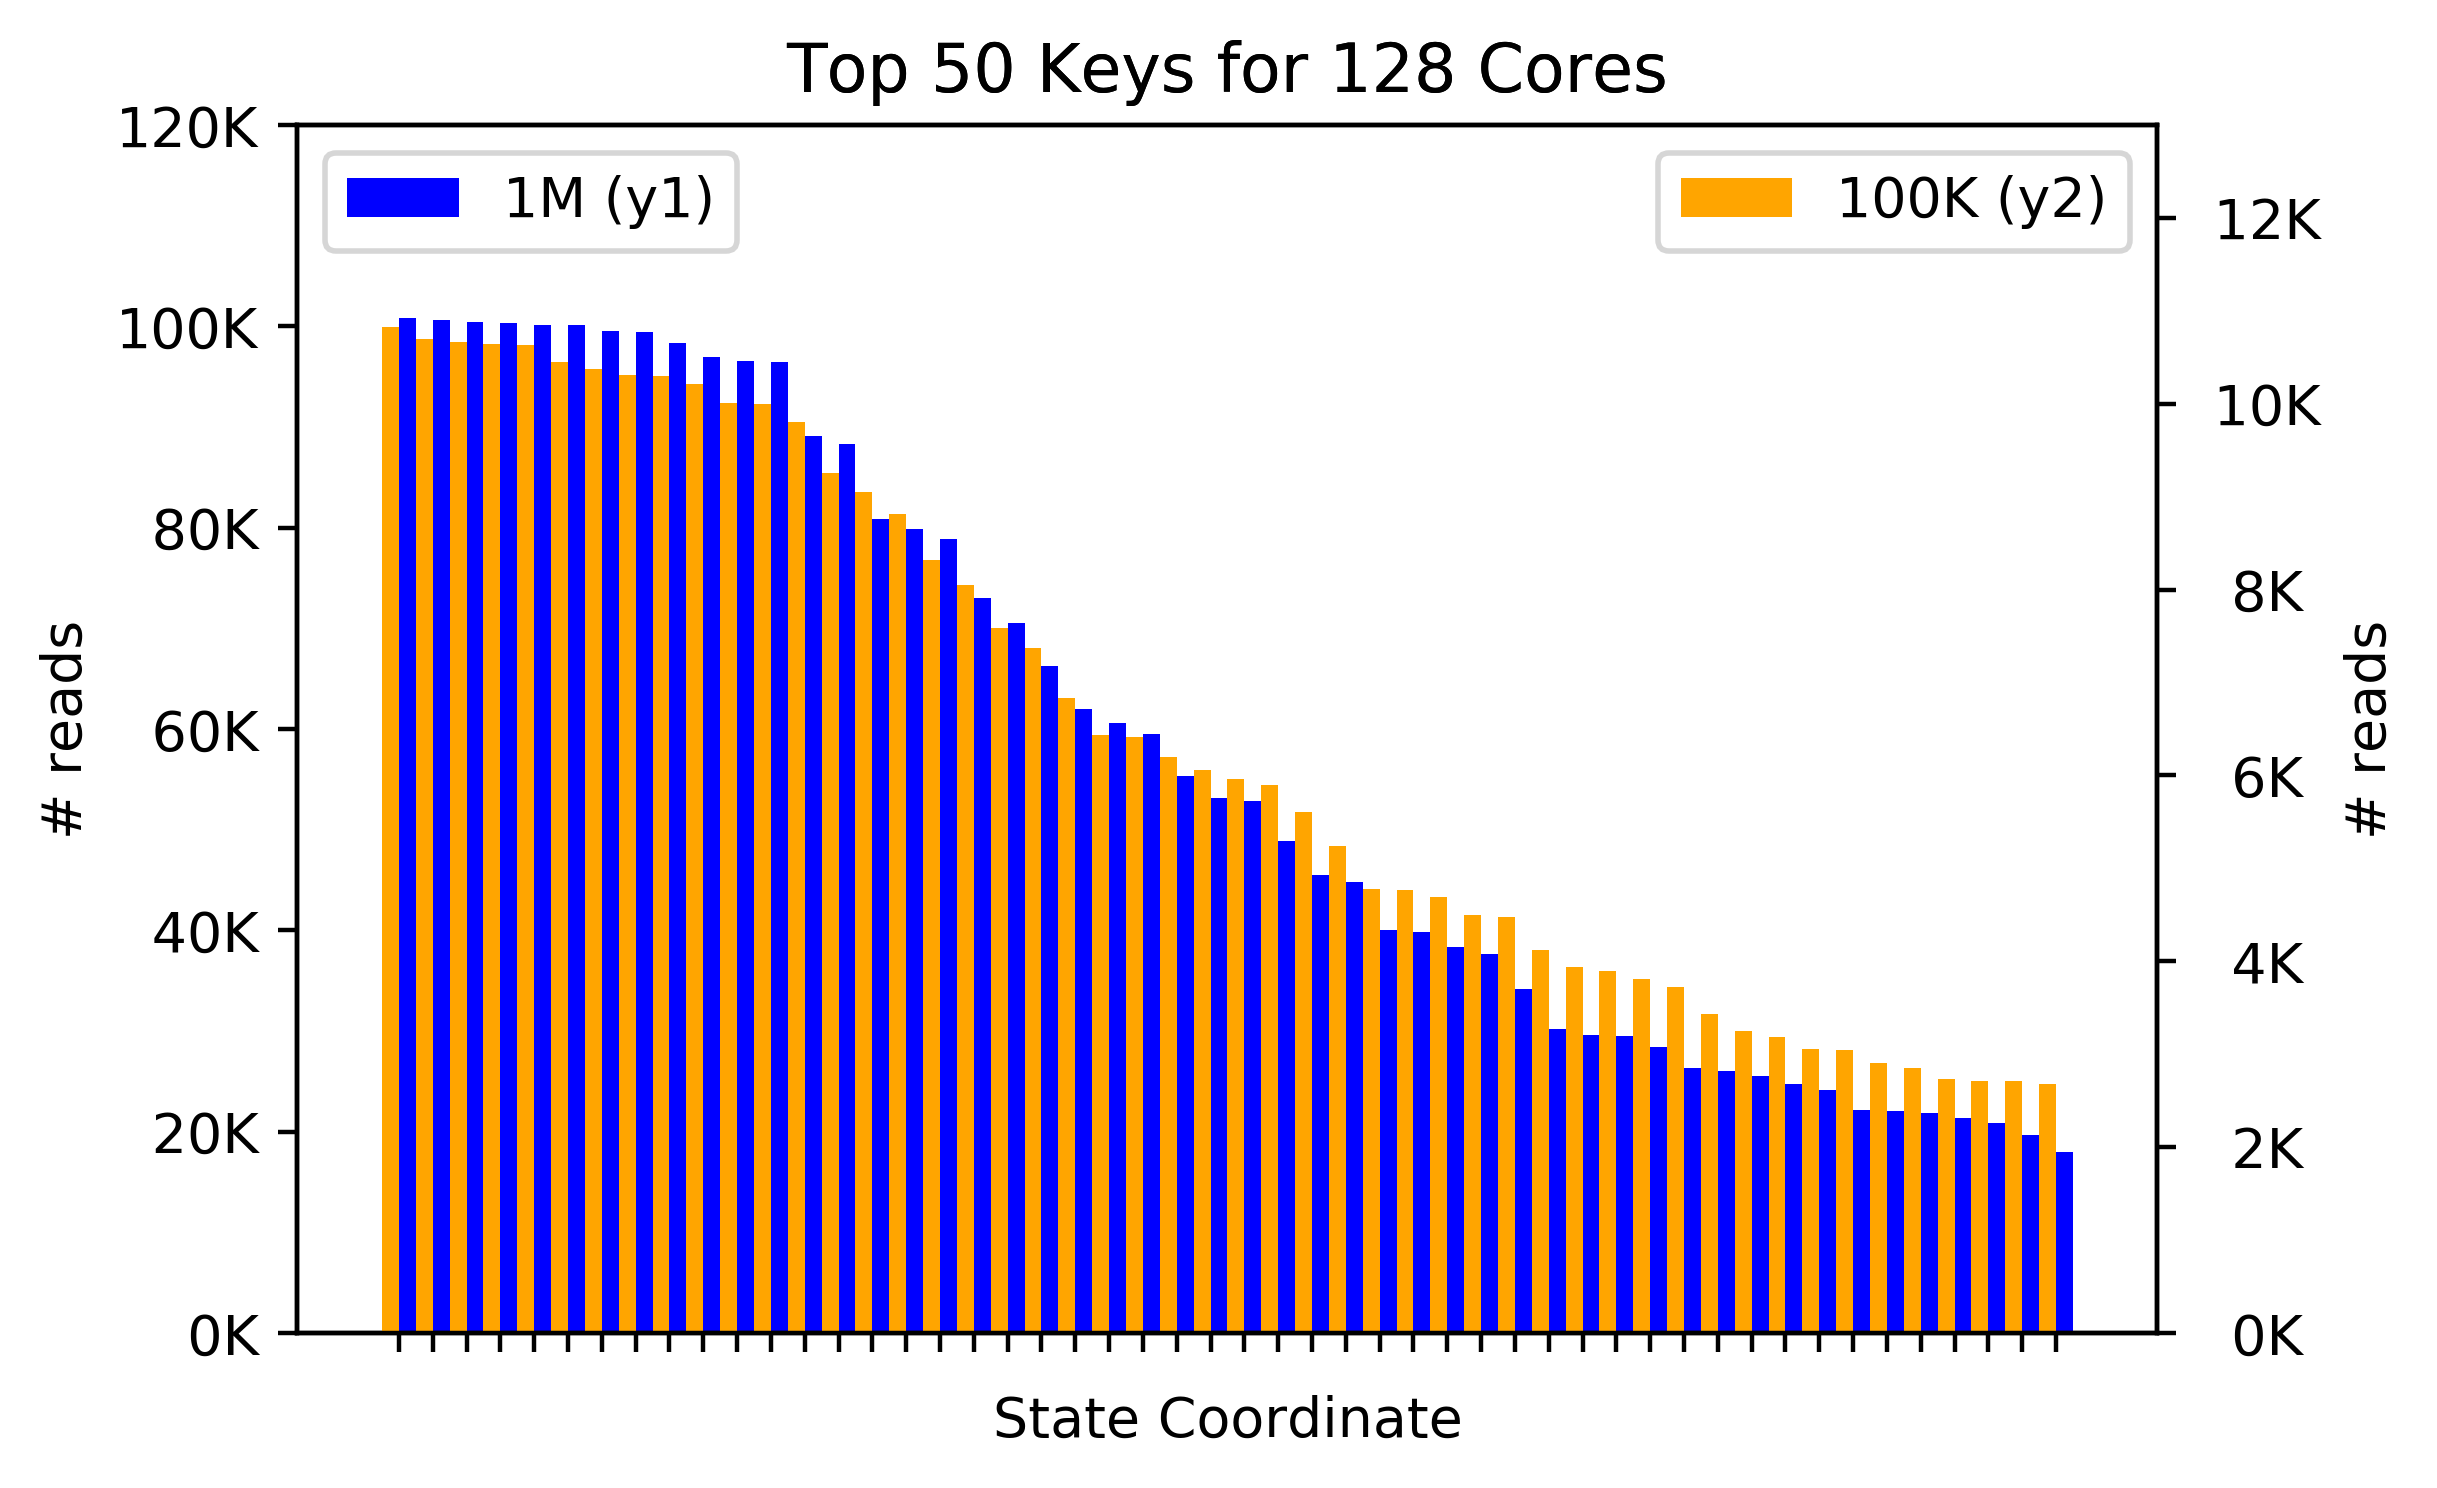
\includegraphics[width=0.45\textwidth]{figures/methodology-keys.png}\\
  \caption{The keyspace imbalance is due to workers generating deep
  trajectories and pulling the same coordinates. Over time, the accesses get
  dispersed across different coordinates resulting in some keys being more
  popular than others.\label{fig:methodology-keys}}
\end{figure}

\subsection{Positive Effects of Load Balancing}
\label{sec:positive-effects-of-load-balancing}

% What did we do
The ``active but small keyspace" encourages replication across a cluster.  To
motivate the need for this type of load balancing we show how limiting the
cache size saves memory and sacrifices neglible performance. This type of
analysis informs our load balancing policies for when we switch to a
distributed key-value store backend to store segment coordinates.  We need to
know when and how to partition the keyspace: a smaller cache hurts performance
because key-value pairs need to be retrieved from other nodes while a larger
cache has higher memory usage. 

% techinical details
On each node, ParSplice uses an infinitely large cache to store segment
coordinates. We limit the size of the cache using an LRU eviction policy, where
the penalty for a cache miss is retrieving the data from the persistent
database.  We check every operation instead of when segments complete because
(1) the cache fills up too fast, and (2) it reduces the overhead of key
eviction. 

% results: cache size trade-offs
The results for different cache sizes for a growth rate of 100K over a 2.5 hour
run is shown in the left two plots of Figure~\ref{fig:methodology-tradeoff}.
``Baseline" is the performance of unmodified ParSplice  measured in trajectory
duration (\(y\)-axis) and utilization is measured with memory footprint (\(y2\)
axis) of just the cache.  ``Static Load Balancing Policies" shares the
\(y\)-axis and shows the trade-off for different cache sizes. The error bars
are the standard deviation of 3 runs. 

% results: raw numbers
Although the keyspace grows to 150K, a 100K key cache achieves 99\% of the
peformance. Decreasing the cache degrades performance and predictability.  Not
suprisingly, the memory usage all decreases with the cache size and although we
only save 0.4GB, larger and more complicated runs use up to 4GB, which is 3\%
of the 128GB on each node. Note that this is an addition to the 30GB that
ParSplice uses to manage other ranks on the same node. While this result
trade-off is not unexpected, it nonetheless achieves our goal of showing the
benefits of load balancing keys across nodes and that smaller caches on each
node are an effective way to save memory without completely sacrificing
performance.

\begin{figure*}[tbh]
  \noindent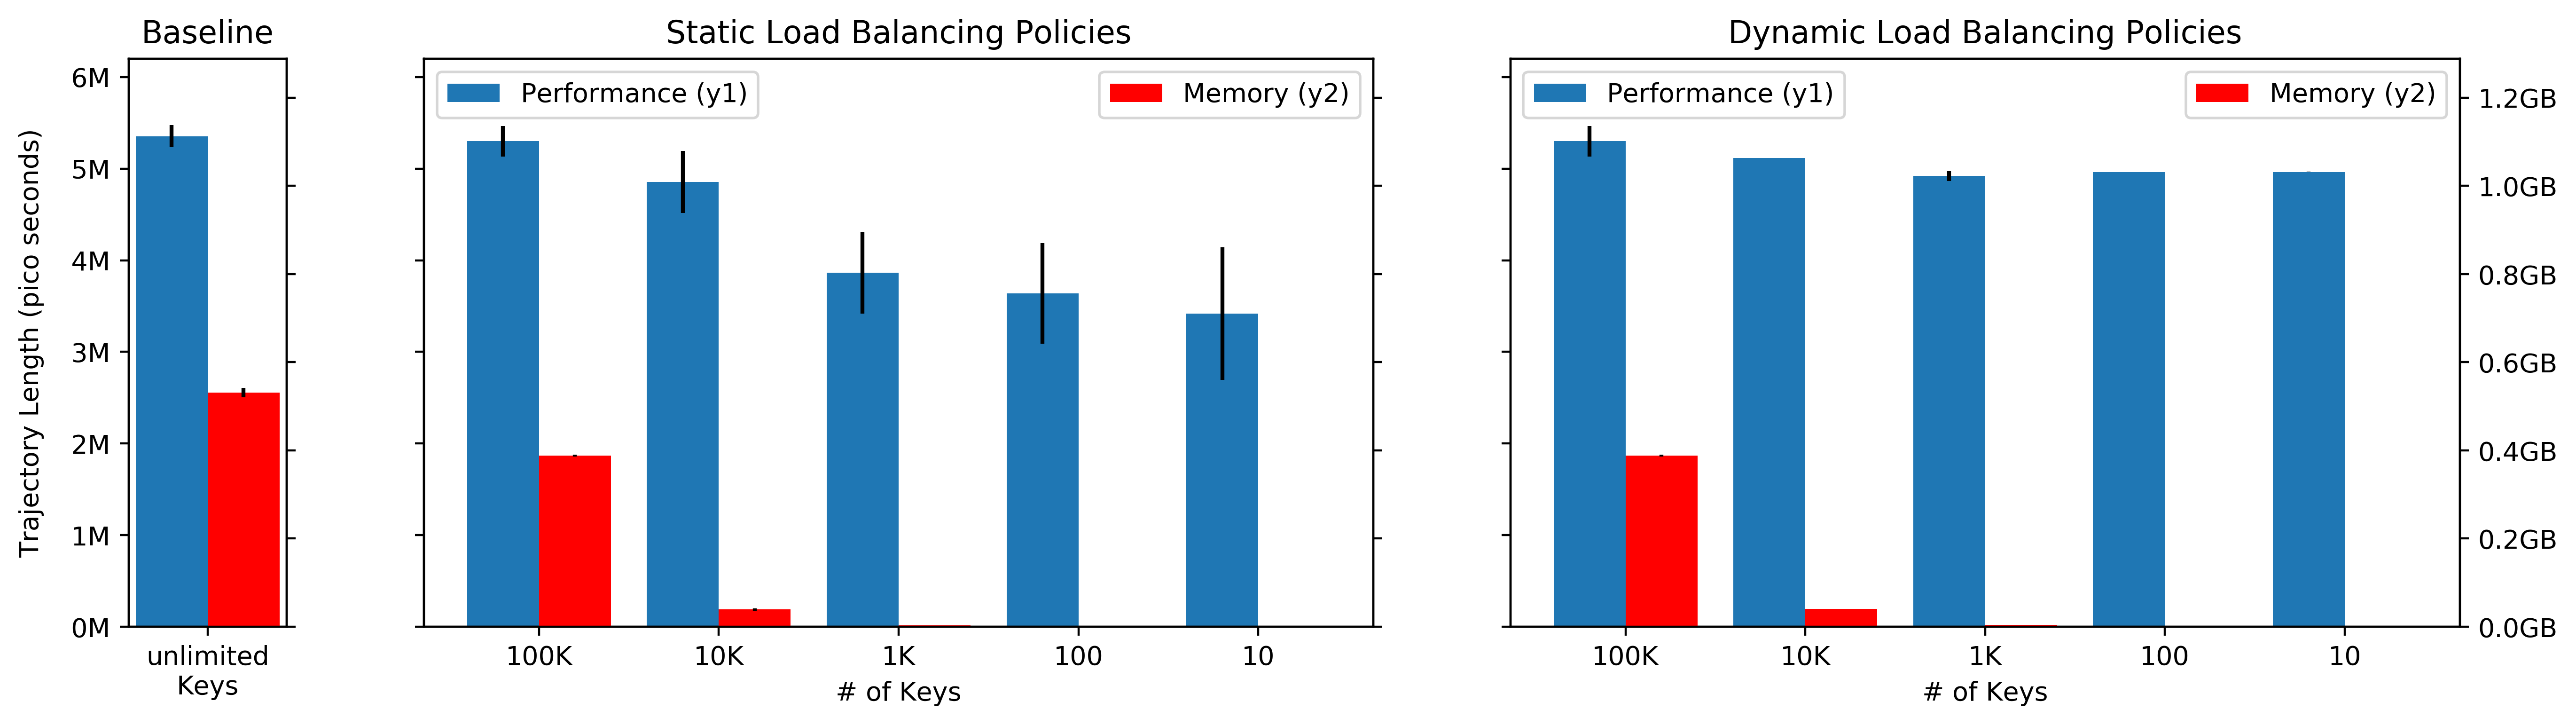
\includegraphics[width=1\textwidth]{figures/methodology-tradeoff.png}\\
  \caption{The optimal cache size must strike a balance between performance and
  resoure utilization. Here we show the trade-off for a static load balancing
  policy that evicts keys when the cache reaches a certain size. For this
  configuration, a 100K key cache has the best performance/utilziation, despite
  the keyspace being 250K keys. \label{fig:methodology-tradeoff}}
\end{figure*}

\subsection{The Need for Dynamic Load Balancing Policies}

% why is the performance lower for smaller caches?
Despite the memory savings, our results suggest that dynamic load balancing
policies could save even more memory.  The left two plots in
Figure~\ref{fig:methodology-tradeoff} show that a 100K key cache is sufficient
as a static policy but the top graph in Figure~\ref{fig:futurework-regimes}
indicates that the value should be much smaller. That graph shows that the
beginning of the run is characterized by many reads to a small set of keys and
the end sees much lower reads per second to a larger keyspace. Specifically, it
shows only about 100 keys are active in the latter half of the run, so a
smaller cache should indeed suffice. After analyzing traces, we see that the
100 key cache is insufficient because LevelDB cannot service the read-write
traffic. By limiting the size of the cache, some reads must traverse up the
ParSplice cache hierarchy to the persistent database (in this case, LevelDB).
According to Figure~\ref{fig:futurework-regimes}, the read requests arrive at
750 reads per second in addition to the writes that land in each tier (about
300 puts/second, some redundant). This traffic triggers a LevelDB compaction
and reads block and eventually pile up, resulting in very slow progress. Traces
verify this hypothesis and show reads getting backed up as the read/write ratio
explodes. To recap, small caches incurr too much load on LevelDB at the
beginning of the run but smaller caches should suffice after the initial read
flash crowd passes because the keyspace is far less active, so we need a two
part load balancing policy.

% what is mantle
To explore dynamic load balancing policies, we use the Mantle approach.  Mantle
is a framework buit on the Ceph file system that lets admnistrators control
file system metadata load balancing policies. The basic premise is that load
balancing polcies can be expressed with a simple API consisting of when, where,
and how much callbacks. The succinctness of the API lets users inject
muitiple, dynamic policies.  

% Why is this a good idea
Although ParSplice does not use a distibuted file system, its workload is very
similiar because the minima key-value store responds to small and frequent
requets, which results in hot spots and flash crowds.  Distributed file systems
solve similiar issues: since data IO does not scale like metadata
IO~\cite{roselli:atec2000-FS-workloads}, finding optimal ways to measure,
migrate, and partition metadata load is a relatively new field, but has been
shown to lead to large performance increases and more scalable file
systems~\cite{zheng:pdsw2014-batchfs, grider:pdsw2015-marfs,
ren:sc2014-indexfs, patil:fast2011-giga+, brandt:msst2003-lh}.  Both workloads
also have data locality so the storage should have mechanisms for leveraging
requests with similar semantic meaning.  Previous work shows that Mantle speeds
up file systems by making metadata access faster, leveraging the fact that file
system metadata IO imposes small and frequent accesses on the underlying
storage system.  

% why is it awesome.
%Mantle controls how to distribute or concentrate file system metadata and helps
%users quantify the effects of load balancing.  The paper identified effective
%file system load balancing policies and tested them under metadata-intensive
%workloads. The Greedy Spill balancer, which was based
%on~\cite{patil:fast2011-giga+}, sheds half its load aggressively when there are
%avaiable servers.  The Fill and Spill balancer, which was based
%on~\cite{pai:asplos1998-lard} sheds a fraction of the load only when the server
%is overloaded. Finally, the Adaptable balancer, which was based
%on~\cite{weil:sc2004-dyn-metadata, weil:osdi2006-ceph}, sheds a fraction of the
%load frequently. Mantle is also a powerful debugging tool.

%HXHIM is a good fit because it has migration mechanisms for load balancing
%\begin{itemize} \item bulk operations (\texttt{put/get()}) \item key
%partitioners \item secondary indices \end{itemize} \item we need a way to
%learn these regimes \begin{itemize} \item Figure~\ref{keyspace-regimes-4hr}
%shows the same phases as 100K but that the timestamps affected by delay
%\end{itemize} \end{itemize}
%
% What is Mantle?
% How does it work?
%It was built on CephFS, the file system above Ceph, so it inherits many of
%characteristics of the CephFS architecture, like the dedicated metadata cluster
%and heartbeat mechanisms shown at the top of Figure~\ref{fig:arch-mantle}.
%Each metadata server manages differently sized subtrees of the logical
%namespace and migration decisions are made synchronously, every 10 seconds.
%CephFS already had the mechanisms for load balancing, namely the ability to
%measure the load on a subtree, to migrate subtrees, and to partition subtrees
%into smaller subtrees, but it had hard-coded, ad-hoc policies for guiding the
%migrations.  Mantle reads user-defined policies written in Lua and returns
%decisions for how load should be migrated given the state of the cluster and
%the behavior of the workload. The hooks in Figure~\ref{fig:arch-mantle} show
%where CephFS calls out to the Mantle library to make decisions. While the
%decisions were made by Mantle, CephFS used its internal mechanisms to do the
%load balancing.

% What is the status?
%It was merged\footnote{https://github.com/ceph/ceph/pull/5155} and is starting
%to get users who are frustrated with the hard-coded load balancing policies
%that are shipped with CephFS. It was re-implemented using the ``programmable
%storage" approach~\cite{sevilla:eurosys17} to reduce lines of code for doing
%things like versioning and distributing balancer version.  Although Mantle is
%heavily integrated the daemons that compose an Ceph cluster, using Ceph's
%naming conventions and internal libraries like Ceph's version of protocol
%buffers, there is no reason that it cannot be extracted.
%
%\begin{figure}[tb]
%  \noindent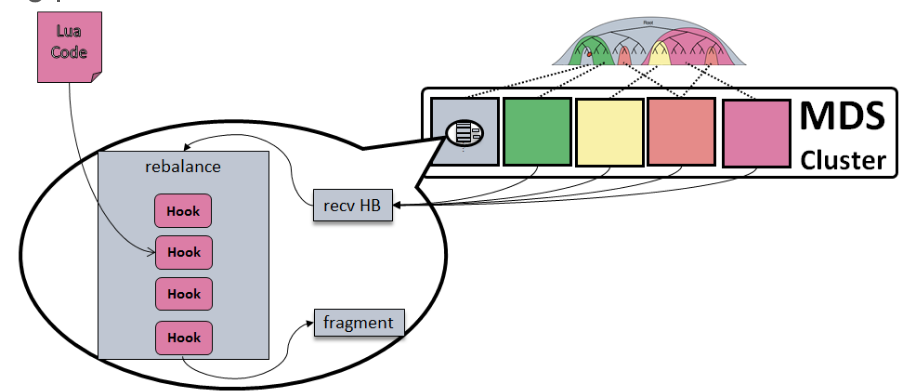
\includegraphics[width=19pc,angle=0]{figures/arch-mantle.png}\\
%  \caption{The Mantle API lets adminstrators control load balancing by
%  changing the poicies for how to distribution or concentrate file system
%  metadata. It was merged into CephFS and inherits many aspects of that
%  architecture. Although it has the load balancing structure and logic from
%  CephFS (gray boxes), the actual API is not dependent on that code base.}
%  \label{fig:arch-mantle}
%\end{figure}
%\begin{figure}[tb]
%  \noindent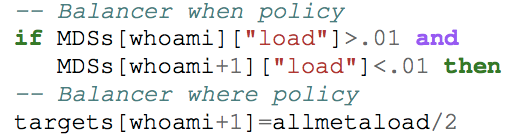
\includegraphics[width=19pc,angle=0]{figures/arch-mantle-example.png}\\
%  \caption{The Greedy Spill balancer written in Lua using the Mantle API.}
%  \label{fig:arch-mantle-example}
%\end{figure}
%

The right most graph of Figure~\ref{fig:methodology-tradeoff} shows the results
of using the Mantle API to program  a dynamic load balancing policy with two
phases into ParSplice:

\begin{itemize}
  \item unlimited growth: cache increases on every put
  \item \(n\) key limit: cache maintained at this size
\end{itemize}

We trigger the policy switch at 100K keys to absorb the flash crowd at the
beginning of the run. Once triggered, keys are evicted to bring the size of the
cache down to the threshold and the least recently keys are actively evicted.
In that figure, the cache sizes are along the \(x\)-axis.

% results: same level of performance can be achived 
The dynamic policies show better performance than the single \(n\) key
policies. The performance and memory utilization for 100K is the same as the
100K bar in the middle graphs but the rest reduce the size of the keyspace
after the read flash crowd. This reduced the read/write traffic on the
persistent database and reduces the amount of stalls.  The worst performing
policy is the 10 key cache, which achieves 94\% of the performance while only
using 40KB of memory. 

% caveats: it is calculating 90% of the trajectory, memory value reported is final
\subsubsection*{Caveats}

The results from the right most graph in Figure~\ref{fig:methodology-tradeoff}
are slightly deceiving for three reason: (1) segments take longer to generate
later in the run, (2) the memory footprint is the value at the end of 2.5
hours, and (3) this policy only works well for the 2.5 hour run.  For (1), the
curving down of the simulation vs. wall-clock time is shown in
Figure~\ref{fig:methodology-trajectory}; as the nanoparticle grows it takes
longer to generate segments so by the time we reach 2.5 hours, over 90\% of the
trajectory is already generated.  For (2), the memory footprint is around 0.4GB
until we reach 100K keys. In Figure~\ref{fig:methodology-tradeoff} we plot the
final value. For (3), Figure~\ref{fig:methodology-trajectory} shows that the
cache fills up with 100K keys at time x and its size is reduced to the size
listed in the legend.  The curves stay close to ``Unlimited" for up to an hour
after the cache is reduced but eventually flatten out as the persistent
database gets overloaded. 10K and 100K follow the ``Unlimited" curve the
longest and are sufficient policies for the 2.5 hour runs but anything longer
would need a different dynamic load balancing policy.

\begin{figure}[tbh]
  \noindent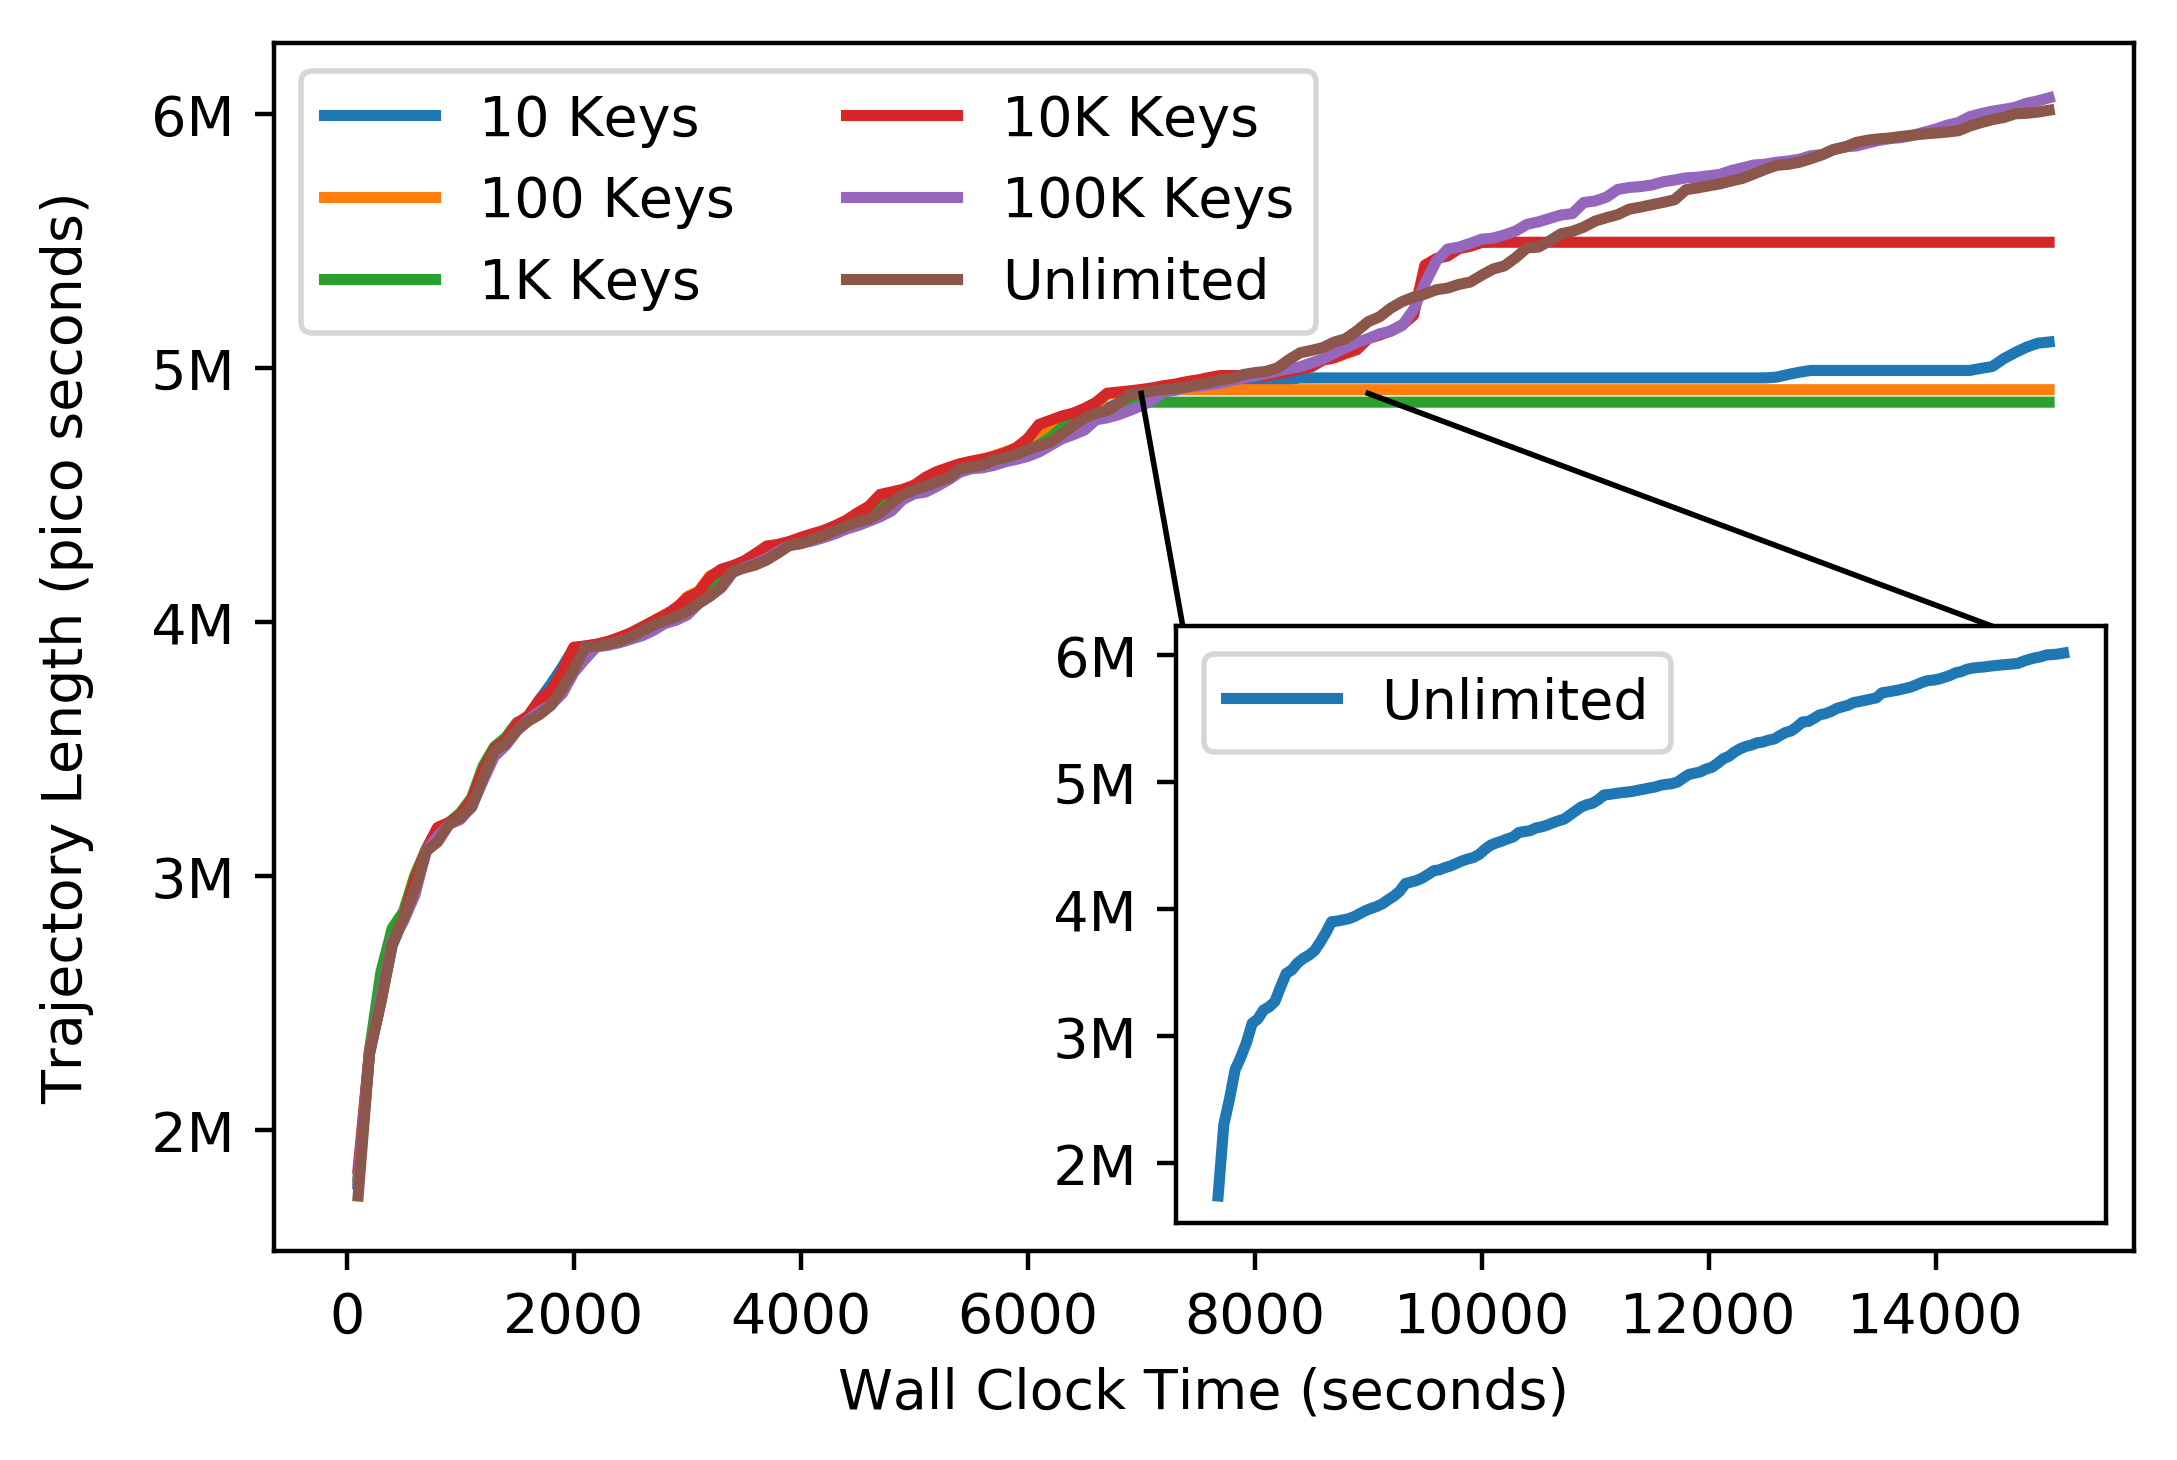
\includegraphics[width=0.45\textwidth]{figures/methodology-trajectory.png}\\
  \caption{The optimal cache size must strike a balance between performance and
  the keyspace being 250K keys. \label{fig:methodology-trajectory}}
\end{figure}

% wht the result is still valie
Despite these caveats, the result is still valid: we found a dynamic load
balancing policy that absorbs the cost of a high read throughput on a small
keyspace and reduces the memory pressure for a 2.5 hour run. The problem is
that the thresholds in these policies does not work for different setups ({\it
i.e.} different ParSplice parameters, number of worker nodes, and job lengths).
We need a way to identify what thresholds we should use for different job
permutations.


\subsection{Machine Learning Keyspace Activity}

We can't find the optimal keypsace size for every permuation, finding the key threshold changes with
\begin{itemize}
  \item number of nodes
  \item delay: Figuree~\ref{fig:futurework-regimes}
  \begin{itemize}
    \item unique keys increase over time, throughput of keys goes down
    \item smaller delay has bigger keyspace but keys are way colder 
  \end{itemize}
\end{itemize}


%\begin{itemize}
%  \item C bindings for Mantle
%\end{itemize}
%
%\subsection{Pluggable Interfaces}
%
%\begin{figure}[tb]
%  \noindent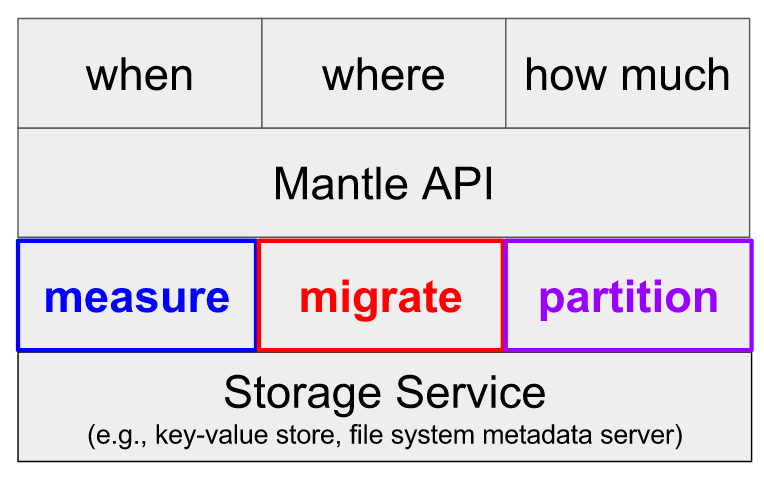
\includegraphics[width=19pc,angle=0]{figures/mantle-pluggable-interfaces.png}\\
%  \caption{The storage service must: \textcolor{blue}{\textbf{measure}}
%  resource usage, \textcolor{red}{\textbf{migrate}} resources, and
%  \textcolor{purple}{\textbf{partition}} resources. }
%  \label{fig:mantle-pluggable-interfaces}
%\end{figure}
%
%\subsubsection{Measure}
%
%The metrics measured should help the system decide ``when" to migrate server
%load. They should:
%
%\begin{itemize}
%  \item tell us about the state of the server or cluster
%  \item provide some value of load, so we can partition/send it
%\end{itemize}
%
%In Ceph: global and local metrics ({\it e.g.}, CPU utilization, file system operation counts) \\
%
%In HXHIM: ???\\
%
%\subsubsection{Migrate}
%
%In Ceph: \texttt{export\_dir()}
%
%In HXHIM: \texttt{mdhimBPut()}, \texttt{mdhimBGet()}, ``adjusting ... keys" ???
%
%\subsubsection{Partition}
%
%In Ceph: subtrees and directory fragments
%
%In HXHIM: secondary indices, cursor types, bul operations
